%   Filename    : chapter_1.tex 
\chapter{Introduction}
\label{sec:researchdesc}    %labels help you reference sections of your document

\section{Overview of the Current State of Technology}
\label{sec:overview}
The Department of Environment and Natural Resources (DENR) expressed on its website that monitoring air quality is essential in reducing air pollution and they plan to protect the environment and public health by strengthening their air quality monitoring systems \cite{DENR2020}.

An example of an air quality monitoring system that the DENR uses is the Differential Optical Absorption Spectroscopy (DOAS)\cite{DENR_ND}. DOAS captures light that passes through the atmosphere, to measure different wavelengths that were absorbed by different gasses. This method can accurately measure trace gasses absorption and it is simpler and less expensive to operate. DOAS, however, is greatly affected by turbulence in the atmosphere \cite{PlattEtAl2008}. DENR also has particulate matter stations that record $PM_{2.5}$ and $PM_{10}$ in the atmosphere \cite{DENR_ND}.

DOAS equipment needs frequent maintenance to be able to operate normally. In a news report by Enano \& Subingsubing \citeyear{enano_subingsubing_2019} regarding air pollution at EDSA it was stated that the maintenance of this equipment requires “hundreds of thousands of pesos”.

Currently, the way to access the data from the AQMS stations is through the website (https://air.emb.gov.ph/ambient-air-quality-monitoring/) and the Google Play Store application. Figure \ref{fig:PAQIApp} shows the contents of the application.\\

  
%--- the following example shows how to include a figure in PNG format
\begin{figure}[!htbp]              %-- use [t] to place figure at top, [b] to place at the bottom, [h] for here
   \centering                    %-- use this to center the figure
   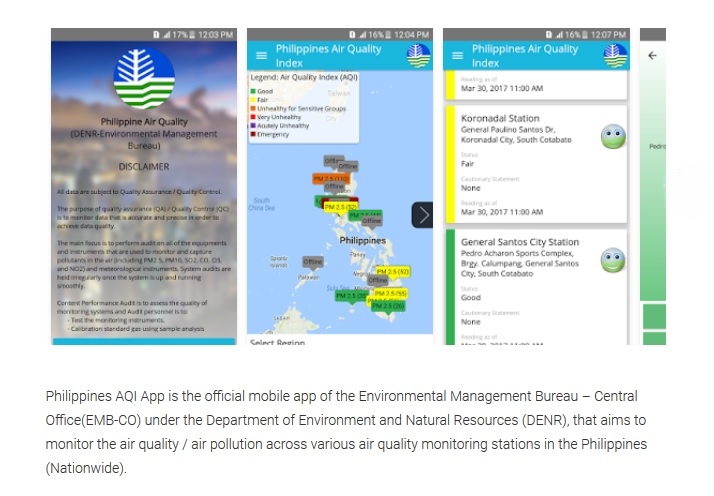
\includegraphics[width=120mm,scale=1.5]{PAQIApp.jpg}      %-- include image file named as "disneychart.png" 
   \caption{Screen capture of the mobile application of the Philippines Air Quality Index.
}
    \label{fig:PAQIApp}
\end{figure}
\FloatBarrier

In the mobile application disclaimer, it is stated that the system audits are irregular and all data are subject to quality assurance and quality control. This means that the end user may not get the accurate data that they expect when using the application. Furthermore, monitoring stations are not online 24/7 which makes the data less accessible.

Aside from DOAS, other novel forms of air quality monitoring systems were developed for similar reasons as the existing technology being expensive. Such is the case for the study of Garcia-Gonzalez et al. \citeyear{GARCIAGONZALEZ2021107950}, wherein they used IP cameras already installed throughout the city of Montreal, Canada, and utilized object detection models to estimate the pollution coming from vehicles. The calculation of the pollution was mainly based on the vehicle’s speed that circulate in the region where the camera is pointed at.

Moreover, there have been efforts to quantify the flow of vehicles in traffic and convert this information into emissions and energy use estimates. A local study by Rito et al.\citeyear{rito_lopez_biona_2021} demonstrated a method of estimating a vehicle’s emission and energy use during transportation by using crowdsourced data from Google Maps. Pollutants such as \ch{CO2} and $PM_{2.5}$ were estimated from vehicles such as tricycles and jeepneys, which contributes to the availability of pollutant data in the country.

In response to the limitations of the currently existing methods of collecting air pollution data, the researchers aimed to develop a cost-effective system that utilizes the current technology such as object detection to estimate pollutant emissions from vehicles in the Philippines. The system, using recently gathered data from vehicles in the country, shall provide an immediate calculation of the pollutant data to be displayed when used. A latent effect of this study shall also contribute to increasing data on images of vehicles that are found locally in the country.



\section{Problem Statement}
	Air pollution has become a global problem over the years. As stated by Akimoto \citeyear{Akimoto2004}, the availability of the \ch{CO2} concentrations on the Measurement of Air Pollution from Satellite (MAPS) instrument in 1981 shows high concentrations of the greenhouse gas over tropical Asia, Africa, and South America. Not only does this data provide evidence that this has become an international issue,  but it also shows how fossil fuel combustion can have an impact on air quality. 

The Philippines, a country located in tropical Asia, is not devoid of these issues. An article by Abano \citeyear{abano_2019} states that a 2018 study by the World Health Organization reports the Philippines has ranked third among the countries with air pollution-related deaths. These deaths are tied to harmful particles entering a person’s lungs, which can lead to multiple different ailments and diseases: heart disease, lung cancer, and respiratory infections, to name a few.

Air pollution can come from different sources, whether it be from stationary constructs like factories or mobile sources such as cars \cite{EMB_2015}. An air quality status report by the Department of Environment and Natural Resources (2015) shows that 65\% of air pollutants come from these mobile sources. This worsened as the EMB’s official site, Environmental Management Bureau \citeyear{EMB_2018}, states that based on the Emissions Inventory of 2018, the pollutant contribution of mobile sources has increased to  74\%. In places where traffic is congested could be a huge contributing factor to vehicular emissions. Vergel and Yai \citeyear{vergel_yai2000} state that the congestion in the roads of Metro Manila contributes to the worsening air quality, especially in the vicinity of the road environment.

A key component of these emissions is particulate matter ($PM$): $PM_{2.5}$ and $PM_{10}$. $PM$ is a measure of solid or liquid particles in the air that are inhalable, this includes dust, smoke, and dirt \cite{EPA_2022}. Accordingly, $PM_{10}$ is the measure of inhalable particulate matter in the air that is at most 10 micrometers in diameter. Similarly, $PM_{2.5}$ is the measure of inhalable particulate matter in the air that is at most 2.5 micrometers in diameter. United States Environmental Protection Agency (US EPA) \citeyear{EPA_2022} additionally states that microscopic particulate matter particles can be inhaled and cause them to get to the lungs or the bloodstream which can lead to serious health problems, with $PM_{2.5}$ having the greatest risk.

Other components of emissions that contribute to pollution are greenhouse gases. These gases are Carbon Dioxide (\ch{CO2}), Nitrous Oxide (\ch{N2O}), and Methane (\ch{CH4}). According to US EPA \citeyear{EPA_2023}, Carbon Dioxide is produced by burning fossil fuels, solid waste, trees, and other biological materials; which then enters the atmosphere. The site further defined Methane as gas the is emitted during the "production and transport of coal, natural gas, and oil." Lastly, Nitrous Oxide is another gas that is emitted during the "combustion of fossil fuels and solid waste." These greenhouse gases can be an issue to the country as they continue to increase in volume and trap heat in the atmosphere.

In the country’s attempt to mitigate the atmospheric issues, the Philippine Clean Air Act of 1999 (Republic Act No. 8749) was passed \cite{FAO}. It entails the resolution of creating a national program of air pollution management, mainly focusing on pollution prevention. Two decades later and the country still sees increasing pollutants in the air and does not show signs of the improvement that was planned.

Considering that the available technology dedicated to monitoring the air quality in the country can be of help with the Philippine Clean Air Act, yet is sparsely spread throughout the country, this poses problems with the availability of information such as air quality in specific areas in the country. In addition, the scope of information taken from systems such as DOAS is limited to the overall pollutants in the air. Information on vehicular pollutant emissions is frequently not present from air monitoring sites when air quality information is displayed.

With the aforementioned said, a system that could calculate and estimate vehicular emissions can be developed using new technologies to contribute to the monitoring of the air pollutants in the country. Thus, Ha.Zee, a system that can gather pollutant estimation from vehicles, was developed by integrating machine learning and computer vision methods in response to the lack of information availability.



\section{Research Objectives}
\label{sec:researchobjectives}

\subsection{General Objective}
\label{sec:generalobjective}


The general objective of the study was to develop an application that estimates the location’s average amount of  pollutant emission from vehicles through the use of a vehicle detection system via computer vision. This system identified the vehicles on the street from a video recording. The system integrated the $PM_{2.5}$, \ch{CH4}, \ch{N2O}, and \ch{CO2} values of different vehicles. These values were then assigned to their respective vehicle classes to be used for calculating the total average based on the amount of the vehicles present in the footage. The average values of each pollutant were then displayed on the corner of the system's display window for the user to see.



\subsection{Specific Objectives}
\label{sec:specificobjectives}

%
%  \begin{comment} ... \end{comment} is used for multiple lines of comment
%
This study specifically aims to:


\begin{comment}
% IPR acknowledgement: the following sentences and examples are from Ethel Ong's slides 
%     on Research Objectives
How to formulate your research objectives:
1. Identify what research steps do you need to perform to achieve your general objective.
2. Identify the questions that must be answered for you to achieve your general objective.
    Thereafter, convert these questions into action statements

Example #1:

Research Question:
  What are the general features of a web-based learning environment?

Specific Objective:
   To review existing web-based learning environment that teaches language learning for children


Example #2:

Research Question:
   How will you represent commonsense knowledge for use by computer systems?

Specific Objective:
   To identify knowledge representation approaches used by existing story generation systems

Example #3:
Research Question:
   What types of storytelling knowledge are needed to generate stories?

Specific Objective:
    To identify the different types of storytelling knowledge used in generating stories

Example #4:
Research Question:
    What machine learning approaches will you utilize?

Specific Objective:
    To determine existing machine learning algorithms [that can be used in training the computer system to detect cyberbullying cases] 

Example #5: Research Question:
    How will your research output be evaluated?

Specific Objective:
    To define evaluation metrics for validating the accuracy of the translation

\end{comment}

%
%  The following are example specific objectives; replace them with your own 
%

\begin{enumerate}
   
   \item Explore object detection algorithms and find the appropriate model to use for the study
   \item Collect images of vehicles to be used and train a system that detects vehicles in traffic footage.
   \item Calculate the estimated pollutant emission ($PM_{2.5}$, \ch{CH4}, \ch{N2O}, and \ch{CO2}) values based on the detected vehicles in the traffic footage
   \item Test the trained model on the video traffic footage 
   

\end{enumerate}


\section{Scope and Limitations of the Research}
\label{sec:scopelimitations}
This study mainly focused on the pollutants ($PM_{2.5}$, \ch{CH4}, \ch{N2O}, and \ch{CO2}) emitted by traffic in the Western Visayas, Philippines, where the researchers reside as of writing the paper. Thus, it was only be set up and used on vehicles that travel within the country. For this reason, this project had some significant difficulties in using existing databases of vehicles that are mainly found locally, with little to no readily available databases existing to be utilized in the study. To avoid said vehicles from not being detected, the researchers opted to take pictures and videos of the vehicles in traffic to be used as training data. 

The study was limited to gathering data of the common vehicles found around the area, which were: Cars, Motorcycles, Utility Vehicles, Trucks, Tricycles, and Jeepneys. To specify, the class of "Utility Vehicles" encompass vehicles such as vans, buses, pick-up trucks, and the modern jeepneys. The distinction between the old and new jeepneys are based on their engines, wherein most old jeepneys use pre-Euro engines \cite{rito_lopez_biona_2021}. Hyundai \citeyear{Hyundai_ph} also stated that modern jeepneys from their company would be utilizing Euro 4-compliant engines. This is assumed for most types for modern jeepneys, hence why the researchers classified them as utility vehicles.

While some vehicles such as bicycles also share the road, they do not use fuel and create the same pollutants stated in the study and as such, are not included in the training of the system. 

 These vehicles were recorded at public roads in the locations of Iloilo City, Iloilo; Bacolod City, Negros Occidental;and Roxas City, Capiz. The traffic footage was recorded on two smartphone cameras during morning hours and were uploaded in Roboflow, a computer vision developer framework for  preprocessing and model training techniques \cite{Bhattacharyya_2020}. This was used to annotate them as their respective vehicle type. 

 $PM_{2.5}$ can come from many different sources. Air Quality Ontario \citeyear{MECP_nd} states that the major sources of  $PM_{2.5}$ are ``motor vehicles, smelters, power plants, industrial facilities, residential fireplaces and wood stoves, agricultural burning, and forest fires." Since this project focuses on detecting vehicles, other objects were not accounted for when calculating the total $PM_{2.5}$ in the vicinity. Thus, this application was limited to finding an estimate of the average $PM_{2.5}$ emissions produced only by vehicles.

Furthermore, this study utilized the YOLOv5 object identification framework and was thus limited to the features of that version. Any other features and upgrades that are present in future versions of the framework were not be included in the study. 



\begin{comment}

%
% IPR acknowledgement: the sentences inside this comment are from Ethel Ong's slides on Scope and Limitations of the Research
%
Generally, one paragraph should be allotted for each of your research objectives.

Each paragraph contains a brief overview of the concept/theory and the purpose of doing the associated objective.

Each paragraph also includes a description of the scope/limitation of your study.

* Please refer to the slides for examples.

\end{comment}


\section{Significance of the Research}
\label{sec:significance}

The main objective of this study was to create an application that helps its users identify the $PM_{2.5}$, \ch{CH4}, \ch{N2O}, and \ch{CO2} level estimations of a traffic congested area through a video over the road. It served as an example of how computer vision can be utilized to get an estimate of the pollutants in an area via identifying the vehicles they come from and the amount of $PM_{2.5}$ they produce. This poses benefits to users that want to acquire information on the pollutant levels in traffic-congested areas. Civilians such as joggers are likely to plan their travel accordingly to avoid areas if $PM_{2.5}$ levels get too high.

For the environmental sector, this study can help contribute to air pollution awareness in the country, in which such data can be utilized when creating plans and protocols to combat the rising concern for the country’s air quality. The system is also open source so it is a benefit for the general public to use without needing a full set of gear to check on pollution levels.

Lastly, as interest in the computer vision field of vehicle identification and recognition systems increases, this study can contribute to future research in said field. The study can be of help to future researchers on the topics of tracking vehicular greenhouse gas emissions. This may also provide data to vehicle image databases through the contribution of the local vehicles (Jeepneys and Tricycles) from the Philippines.




\begin{comment}
If applicable, describe possible commercialization and/or innovation in your research.
\end{comment}


